\documentclass[10pt,pdf,hyperref={unicode}]{beamer}

\usepackage{graphicx}
\graphicspath{{./figs/}}

\mode<presentation> {
	\usetheme{Warsaw}
	  % or ...
	  
	\setbeamercovered{transparent}
  % or whatever (possibly just delete it)
}

\usepackage[english]{babel}
\usepackage[utf8x]{inputenc}

%\usepackage{amsmath}
\usepackage{bm}
\usepackage{tikz}
\usepackage{pgfplots}

\usepackage{color, colortbl}
\definecolor{col1}{gray}{0.8}
\definecolor{col2}{gray}{0.9}
\definecolor{col3}{gray}{0.95}

\title[] % (optional, use only with long paper titles)
{Solution of the 3D Neutron Diffusion Benchmark by FEM}

%\subtitle
%{Include Only If Paper Has a Subtitle}

\author[] % (optional, use only with lots of authors)
{Alexander Avvakumov \inst{1} \and Valery Strizhov \inst{2} \\ 
\and Petr Vabishchevich \inst{2,3} \and \underline{Alexander Vasilev \inst{3}}}
% - Give the names in the same order as the appear in the paper.
% - Use the \inst{?} command only if the authors have different
%   affiliation.

\institute[Universities of Somewhere and Elsewhere] % (optional, but mostly needed)
{
\inst{1} National Research Center "Kurchatov Institute", Moscow, Russia
\\
\inst{2} Nuclear Safety Institute, Russian Academy of Sciences, Moscow, Russia
\\ 
\inst{3} North-Eastern Federal University, Yakutsk, Russia
}

% - Use the \inst command only if there are several affiliations.
% - Keep it simple, no one is interested in your street address.

\date[June 5-9, 2017] % (optional, should be abbreviation of conference name)
{11$^{th}$ International Conference on \\
"Large-Scale Scientific Computations" \\ 
June 5-9, 2017, Sozopol, Bulgaria}
% - Either use conference name or its abbreviation.
% - Not really informative to the audience, more for people (including
%   yourself) who are reading the slides online

\subject{Theoretical Computer Science}
% This is only inserted into the PDF information catalog. Can be left
% out. 

% ����� � ���������
\graphicspath{{./figs/}}
\newcommand{\grad}{\mathop{\rm grad}\nolimits}
\renewcommand{\div}{\mathop{\rm div}\nolimits}
\newcommand{\const}{\mathop{\rm const}\nolimits}

\begin{document}

\begin{frame}
  \titlepage
\end{frame}

{
  \begin{frame}<beamer>
    \tableofcontents
  \end{frame}
}

\section{Introduction}
\begin{frame}{Introduction}
\begin{itemize}
\item
neutron-transport equation (time, energy, spatial and angular variables)
\item
simplified forms, multigroup diffusion approximation
\item
stationary state, critical state of the reactor (local balance between the neutron generation and apbsortion)
\item
spectral problem (Lambda Modes problem, $\lambda$-eigenvalue problem), 
provided that the k-effective is equal to unity, stationary neutron flux is a corresponding eigenfunction 
\item
This work is focused on the solution of the 3D benchmark problem of a VVER-1000 core in steady state. Convergence of the benchmark solution is under investigation.
\end{itemize}
\end{frame}

\section{Problem description}
\subsection{Multigroup diffusion approximation}
\begin{frame}{Multigroup diffusion approximation}
Neutron flux dynamics is considered within a bounded 2D or 3D domain  $\Omega$ ($\bm x = \{x_1, ..., x_d\} \in \Omega, \ d = 2,3$) with a convex boundary $\partial \Omega$. The neutron transport is described by the following set of equations without taking into account delayed neutron sources:
\begin{eqnarray*}
\frac{1}{v_g} \frac{\partial \phi_g}{\partial t} - \nabla \cdot D_g \nabla \phi_g + \Sigma_{rg} \phi_g - \sum_{g\neq g'=1}^{G} \Sigma_{s,g'\rightarrow g} \phi_{g'} = 
\\ 
= ((1-\beta) \chi_g  + \beta\widetilde{\chi}_g) \sum_{g'=1}^{G} \nu \Sigma_{fg'} \phi_{g'} , \quad  g = 1,2, ..., G .
\end{eqnarray*}
Here $\phi_g(\bm x,t)$ is the neutron flux,
$v_g$ is the effective neutron velocity,
$D_g(\bm x)$ is diffusion coefficient, 
$\Sigma_{rg}(\bm x,t)$ is removal cross-section,
$\Sigma_{s,g'\rightarrow g}(\bm x,t)$ is scattering cross-section,
$\nu\Sigma_{fg}(\bm x,t)$ is generation cross-section, 
$\beta$ is the effective fraction of delayed neutrons, 
$\chi_g$, $\widetilde{\chi}_g$  is the spectra of instantaneous and delayed neutrons.
\end{frame}

\subsection{Initial and boundary conditions}
\begin{frame}{Initial and boundary conditions}
The conditions so-called albedo-type are set at the boundary $\partial \Omega$:
\begin{eqnarray*}
 D_g\frac{\partial \phi_g}{\partial n} + \gamma_g \phi_g = 0, \quad 
 \quad g = 1,2, ..., G ,
\end{eqnarray*}
where $n$ is the outer normal to the boundary $\partial \Omega$.

Let's consider problem with albedo boundary conditions and initial conditions
\begin{eqnarray*}
 \phi_g(\bm x,0) = \phi_g^0(\bm x), 
  \quad  g = 1,2, ..., G .
\end{eqnarray*} 

\end{frame}

\subsection{Operator formulation}
\begin{frame}{Operator formulation}
Let's write the boundary problem in operator form. We define the vector $\bm \phi = \{\phi_1, \phi_2, ..., \phi_G\}$ and the matrices
\[
 V = (v_{g g'}),
 \quad v_{g g'} = \delta_{g g'} v_g^{-1},
 \quad
 D = (d_{g g'}),
 \quad d_{g g'} = - \delta_{g g'} \nabla \cdot D_g \nabla,
\] 
\[
 S = (s_{g g'}),
 \quad  s_{g g'} =  \delta_{g g'} \Sigma_{rg} - \Sigma_{s,g'\rightarrow g} ,
\quad
 R = (r_{g g'}),
 \quad  r_{g g'} = ( (1-\beta) \chi_g + \beta \widetilde{\chi}_g) \nu \Sigma_{fg'} ,
\]
\[
g, g' = 1,2, ..., G.
\] 
Using the set definitions, we get boundary problem in operator formulation:
\begin{eqnarray*}
 V \frac{d \bm \phi}{d t} + (D+S) \bm \phi = R \bm \phi .
\end{eqnarray*}  
We solve the Cauchy problem, when $\bm \phi(0) = \bm \phi^0,$  where $\bm \phi^0 = \{ \phi_1^0,  \phi_2^0, ...,  \phi_G^0 \}$.
\end{frame}

\subsection{Spectal problem}
\begin{frame}
To characterize the dynamic processes in a nuclear reactor, which are described by the Cauchy problem, solutions of some spectral problems (see avvakumov2017*). 
Let's consider the solution of the spectral problem, called Lambda Modes problem:
\[
 (D+S) \bm \varphi  = \lambda^{(k)} R \bm \varphi .
\]
This problem is known as the Lambda modes problem for a given configuration of the reactor core.
The minimal eigenvalue is used for characterization of neutron flux, thus 
\[
 k = \frac{1}{\lambda^{(k)}_1}  
\] 
is the effective multiplication factor.
\vfill
\begin{scriptsize}
*Avvakumov, A.V., Strizhov, V.F., Vabishchevich, P.N., Vasilev, A.O.: Spectral
properties of dynamic processes in a nuclear reactor. Annals of Nuclear Energy,
vol. 99, pp. 68--79 (2017)
\end{scriptsize}
\end{frame}

\subsection{Discretization}
\begin{frame}{Finite element method}
Let $H^1(\Omega)$ -- Sobolev space, $v \in H^1$: $v^2$ and $\vert\nabla v\vert^2$ have a finite integral in $\Omega$. For $\bm v = \{v_1, v_2, ..., v_d\}$ define $V^d = [H^1(\Omega)]^d$. For test functions use notations $\bm \xi  = \{\xi_1, \xi_2, ..., \xi_G\}$.\\
In variation formulation we are looking for $\bm \phi \in V^D$ such that:
\begin{eqnarray*}
\begin{split}
\int_{\Omega} \sum_{g=1}^{G} D_G \nabla \phi_g \nabla  \xi_g d\bm x 
+ \int_{\partial \Omega} \sum_{g=1}^{G} \gamma_g \phi_g \xi_g d\bm x
+ \int_\Omega S \bm \phi \bm \xi  d\bm x 
= \lambda^{(k)} \int_\Omega R \bm \phi\bm \xi d\bm x,
\end{split}
\end{eqnarray*}
for all $\bm \xi  \in V^D$.
\\
Let introduce a discrete function spaces $V_h^D \subset V^D$ and define discrete variational problem.

The standard Lagrangian finite elements of degree p =
1, 2 and 3 are used.
\[
\bm{A} \bm{u} = \lambda^{(k)} \bm{B} \bm{u} 
\]
\end{frame}

\section{The test}
\subsection{General description}
\begin{frame}{AER benchmark}
Three-dimensional and two-group approximation, assemblies are homogeneous. 
There are seven material compositions including
\begin{columns}[]
\column{0.5\textwidth}
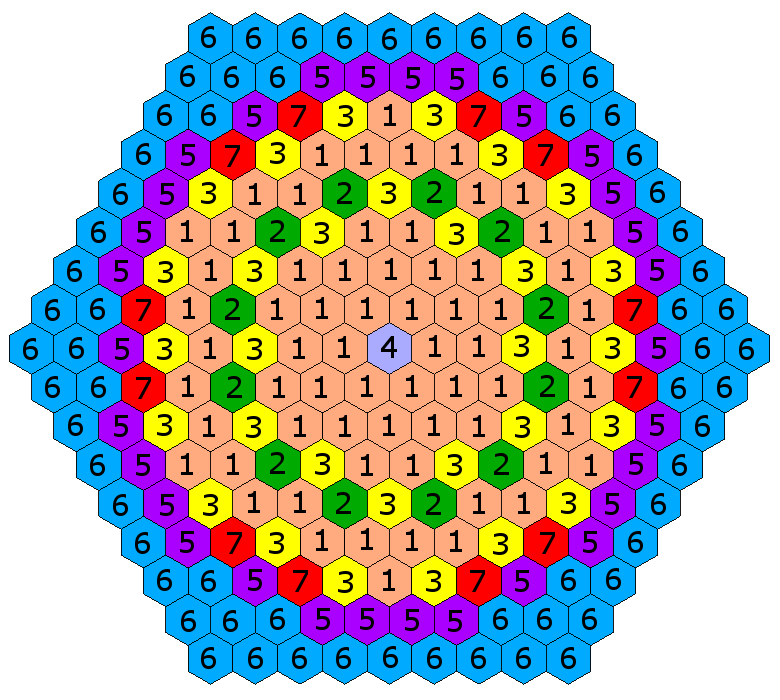
\includegraphics[width=1\linewidth]{1.png}
\column{0.5\textwidth}
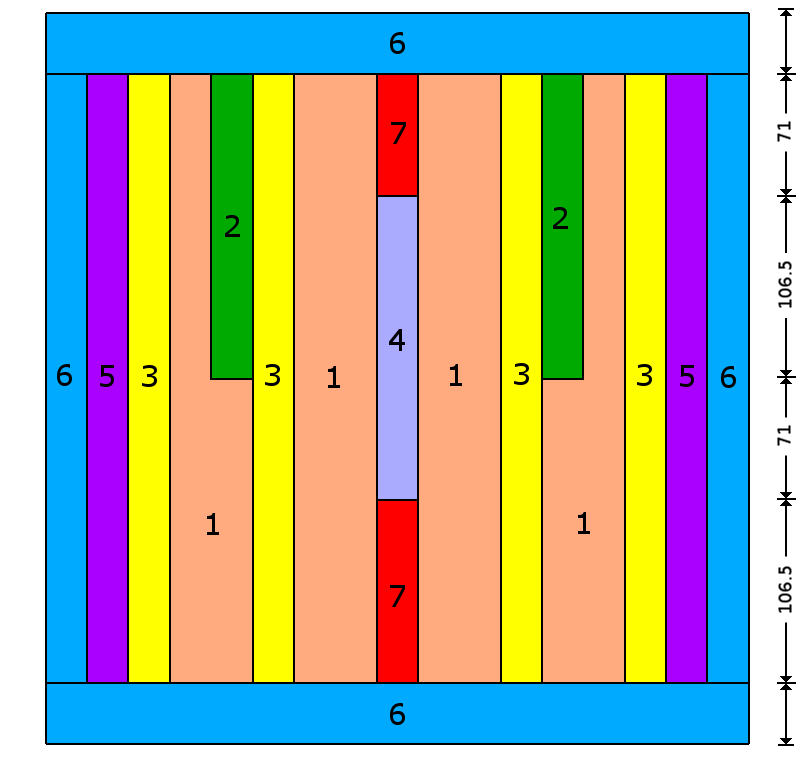
\includegraphics[width=1\linewidth]{2.png}

\end{columns}
\end{frame}

\begin{frame}{mesh and parameters}
\begin{columns}[]
\column{0.5\textwidth}
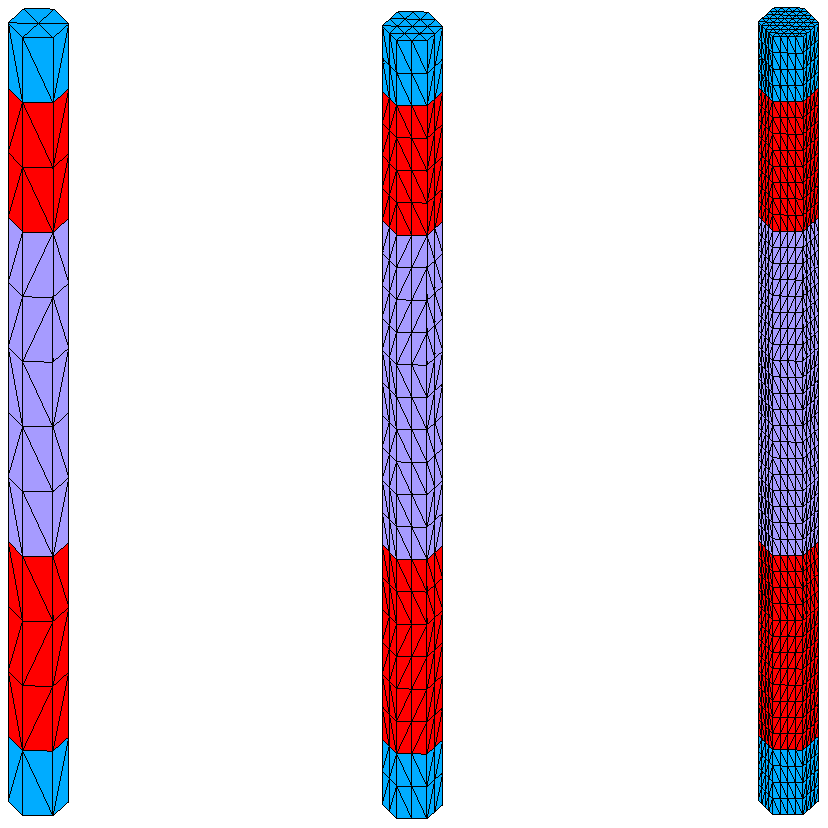
\includegraphics[width=1\linewidth]{3.png}
\column{0.5\textwidth}
In the computations the following parameters  are varied:
\begin{itemize}
\item $\kappa$  from 6 to 96
\item $z$  from 12 to 48
\item$p$  from 1 to 3
\end{itemize}
The following parameters were calculated:
\begin{itemize}
\item the effective multiplication factor $k$;
\item the power distribution  $P$ per assembly:
\[
P = a(\Sigma_{f1} \varphi_1 + \Sigma_{f2} \varphi_2)
\]
\end{itemize}
\end{columns}
\end{frame}

\subsection{Computation parameters}
\begin{frame}{Computation parameters}
The results are compared with those, obtained using the diffusion program CRONOS.

Let's consider the following variations in the calculated parameters:
\begin{itemize}
\item for the effective multiplication factor, absolute deviation from the reference value $k_{ref}$: $\Delta k = |k - k_{ref}|$, expressed in \textit{pcm} (percent-milli, i.e. $10^{-5}$);
\item for power distribution per assembly $P_i$ calculated relative deviation $\varepsilon_i$ (expressed in \%):
\[
\varepsilon_i = \frac{P_i - P_i^{ref}}{P_i^{ref}},
\]
where $P_i^{ref}$ --- reference value of power per assembly $i$ ($i = 1,...,N_e$).
\item by deviations $\varepsilon_i$ calculated integral deviation:
\[
\mathrm{RMS} = \sqrt{\frac{1}{N_e}\sum_{i=1}^{N_e} \varepsilon_i^2}, \quad
\mathrm{AVR} = \frac{1}{N_e}\sum_{i=1}^{N_e} \left\vert \varepsilon_i\right\vert, \quad
\mathrm{MAX} = \underset{i}{\max}\left\vert\varepsilon_i\right\vert.
\]
\end{itemize}
\end{frame}

\subsection{Hardware and Software}
\begin{frame}{Hardware}
\begin{columns}[]
\column{0.6\textwidth}
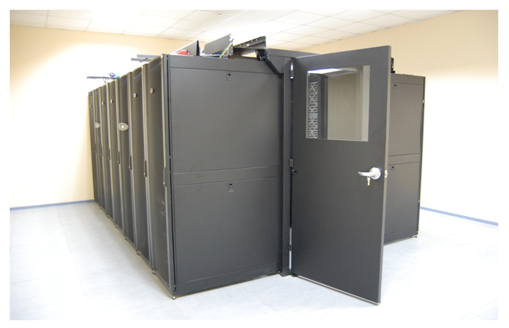
\includegraphics[width=1\linewidth]{cluster.png}
\column{0.4\textwidth}
CPU:
\begin{itemize}
\item 160 nodes (1920 cores)
\item 23.5 TFLOPS (peak), 20.21 TFLOPS (Linpack)
\end{itemize}
GPU:
\begin{itemize}
\item 15 nodes (45 gpu)
\item 22.5 TFLOPS (peak), 11.12 TFLOPS (Linpack)
\end{itemize}
\end{columns}
\end{frame}

\begin{frame}{Software}
\begin{table}[]
%\scriptsize
\begin{tabular}{|c|c|p{5cm}|}
\hline
\textbf{Code section}  & \textbf{Software} & \textbf{\phantom{123456} Description} \\
\hline
Geometry and mesh & Gmsh 3.0.2 & a three-dimensional finite element mesh generator \\
\hline
Eigenvalue & SLEPc 3.7 & the scalable library for eigenvalue problem computations \\
\hline
FEM library & FEniCS 1.6 & a popular computing platform for partial differential equations\\
\hline
Programming & Python 2.7 & a programming language\\
\hline
Visualization &  ParaView 5.4 & a multi-platform data analysis and visualization application \\
\hline
\end{tabular}
\end{table}
\end{frame}

\subsection{Computational results}
\begin{frame}{Eigenvalues for p=1}
\begin{table}[htp]
\small
\caption{$k_1$ results for the Schulz benchmark.}
\label{t-2}
\begin{tabular}{rrrrrrrrr}
\rowcolor{col1}
$p$ & $\kappa$ & $z$ &\multicolumn{1}{c}{$k_1$} & \multicolumn{1}{c}{$\Delta k$} & \multicolumn{1}{c}{MAX} & \multicolumn{1}{c}{AVR}& \multicolumn{1}{c}{RMS}& N \\
\rowcolor{col3}
1& 6& 12& 1.0476057& 192.03& 7.9382& 2.5145& 2.7918& 18,278 \\
\rowcolor{col2}
1& 6& 24& 1.0484070& 111.90& 7.6614& 2.3465& 2.5983& 35,150 \\
\rowcolor{col1}
1& 6& 48& 1.0486511& 87.49& 7.6793& 2.3643& 2.6092& 68,894 \\
\rowcolor{col3}
1& 24& 12& 1.0482940& 123.20& 2.2234& 0.5665& 0.7041& 70,382 \\
\rowcolor{col3}
1& 24& 24& 1.0487937& 73.23& 1.9377& 0.4050& 0.4774& 135,350 \\
\rowcolor{col1}
1& 24& 48& 1.0493645& 16.15& 1.9823& 0.3980& 0.4612& 265,286\\
\rowcolor{col3}
1& 96& 12& 1.0483122& 121.38& 1.2015& 0.3780& 0.4857& 276,146\\
\rowcolor{col2}
1& 96& 24& 1.0490651& 46.09& 0.2647& 0.1129& 0.1389& 531,050\\
\rowcolor{col1}
1& 96& 48& 1.0493997& 12.63& 0.4554& 0.1019& 0.1243& 1,040,858\\
\end{tabular}
\end{table}
\end{frame}

\begin{frame}{Eigenvalues for p=2}
\begin{table}[htp]
\small
\caption{$k_1$ results for the Schulz benchmark.}
\label{t-2}
\begin{center}
\begin{tabular}{rrrrrrrrr}
\rowcolor{col1}
$p$ & $\kappa$ & $z$ &\multicolumn{1}{c}{$k_1$} & \multicolumn{1}{c}{$\Delta k$} & \multicolumn{1}{c}{MAX} & \multicolumn{1}{c}{AVR}& \multicolumn{1}{c}{RMS}& N \\
\rowcolor{col3}
2& 6& 12& 1.0496463& -12.03& 0.9739& 0.4801& 0.5581& 135,350\\
\rowcolor{green}
2& 6& 24& 1.0497290& -20.30& 0.9576& 0.4504& 0.5314& 265,286\\
\rowcolor{col1}
2& 6& 48& 1.0497379& -21.19& 0.9576& 0.4501& 0.5307& 525,158\\
\rowcolor{col3}
2& 24& 12& 1.0494978& 2.82& 0.3246& 0.1577& 0.1861& 531,050\\
\rowcolor{col2}
2& 24& 24& 1.0495665& -4.05& 0.2597& 0.1176& 0.1414& 1,040,858\\
\rowcolor{col1}
2& 24& 48& 1.0495858& -5.98& 0.2435& 0.1117& 0.1335& 2,060,474\\
\rowcolor{col3}
2& 96& 12& 1.0494551& 7.09& 0.1786& 0.0662& 0.0771& 2,103,650\\
\rowcolor{col2}
2& 96& 24& 1.0495265& -0.05& 0.0844& 0.0309& 0.0377& 4,123,154\\
\rowcolor{col1}
2& 96& 48& 1.0495471& -2.11& 0.0573& 0.0256& 0.0298& 8,162,162\\
\rowcolor{col3}
\end{tabular}
\end{center}
\end{table}
\end{frame}

\begin{frame}{Eigenvalues for p=3}
\begin{table}[htp]
\small
\caption{$k_1$ results for the Schulz benchmark.}
\label{t-2}
\begin{center}
\begin{tabular}{rrrrrrrrr}
\rowcolor{col1}
$p$ & $\kappa$ & $z$ &\multicolumn{1}{c}{$k_1$} & \multicolumn{1}{c}{$\Delta k$} & \multicolumn{1}{c}{MAX} & \multicolumn{1}{c}{AVR}& \multicolumn{1}{c}{RMS}& N \\
\rowcolor{col3}
3& 6& 12& 1.0495750& -4.90& 0.2149& 0.0956& 0.1153& 444,962 \\
\rowcolor{col2}
3& 6& 24& 1.0495782& -5.22& 0.2110& 0.0931& 0.1125& 877,898  \\
\rowcolor{col1}
3& 6& 48& 1.0495771& -5.11& 0.2005& 0.0900& 0.1082& 1,743,770\\
\rowcolor{col3}
3& 24& 12& 1.0495406& -1.46& 0.0430& 0.0177& 0.0216& 1,756,982\\
\rowcolor{col2}
3& 24& 24& 1.0495382& -1.22& 0.0317& 0.0123& 0.0146& 3,466,478\\
\rowcolor{col1}
3& 24& 48& 1.0495381& -1.21& 0.0286& 0.0102& 0.0126& 6,885,470\\
\rowcolor{col3}
3& 96& 12& 1.0495357& -0.97& 0.0317& 0.0106& 0.0137& 6,982,418\\
\rowcolor{col2}
3& 96& 24& 1.0495338& -0.78& 0.0211& 0.0092& 0.0110& 13,776,122\\
\rowcolor{col1}
3& 96& 48& 1.0495336& -0.76& 0.0162& 0.0080& 0.0100& ~27,363,530\\
\end{tabular}
\end{center}
\end{table}
\end{frame}

\begin{frame}{Comparison with reference(CRONOS)}
\begin{figure}[htp]
	\begin{center}
    		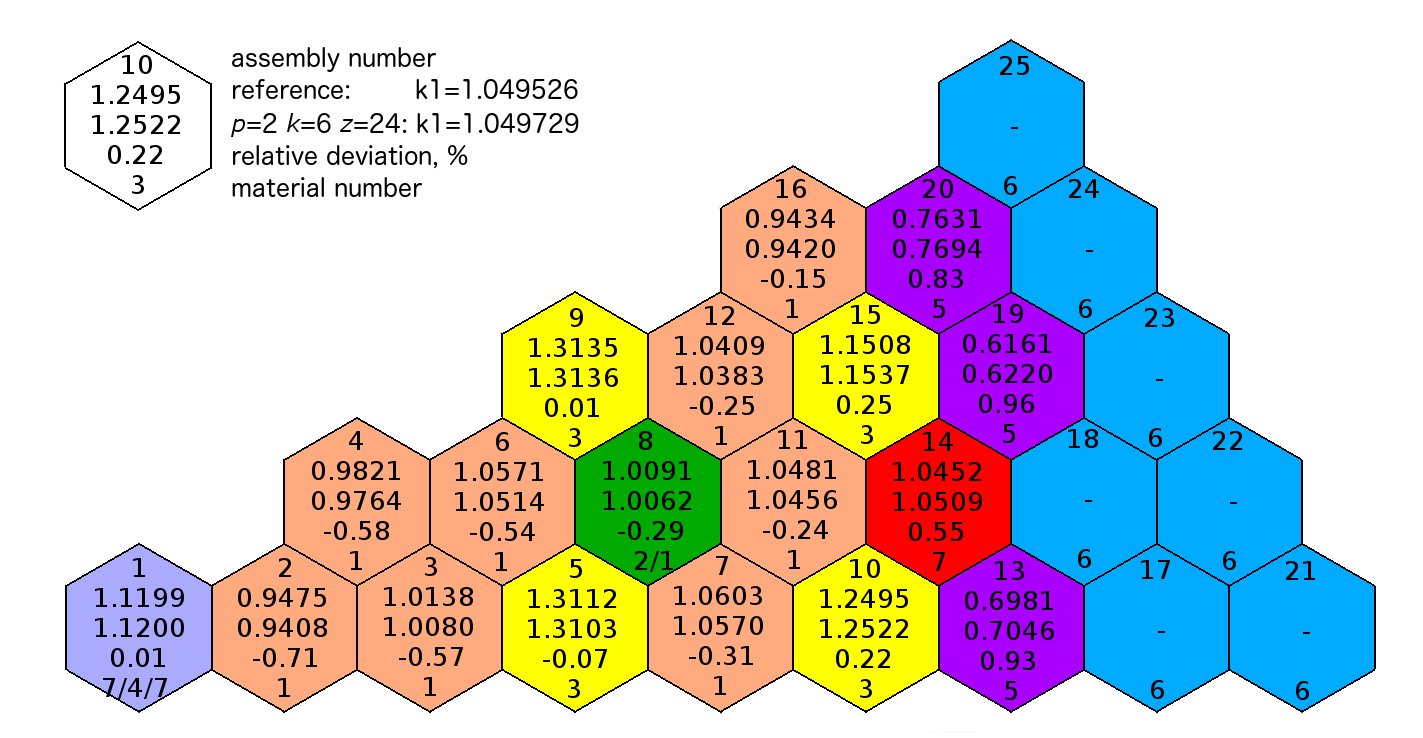
\includegraphics[width=1\linewidth] {power.png}
		\caption{Power distribution at $p=2, \kappa=6, z=24$.}
		\label{fig:3}
  	\end{center}
\end{figure}
\end{frame}

\begin{frame}{Next three eigenvalues}
\begin{table}[htp]
\caption{The eigenvalues $k_2$, $k_3$ and $k_4$.}
\label{t-3}
\begin{center}
\begin{tabular}{rrrrrrr}
\rowcolor{col1}
$p$ & $\kappa$ & $z$ &\multicolumn{1}{c}{$k_2$} & \multicolumn{1}{c}{$k_3$} & \multicolumn{1}{c}{$k_4$} \\
\rowcolor{col3}
1& 6& 12& 1.0367578& 1.0367505& 1.0265919 \\
\rowcolor{col2}
1& 6& 24& 1.0378381&	1.0378355&	1.0286801 \\
\rowcolor{col1}
1& 6& 48& 1.0381457&	1.0381434&	1.0292950\\
\rowcolor{col3}
1& 24& 12& 1.0378816&	1.0378762&	1.0277542\\
\rowcolor{col3}
1& 24& 24& 1.0389665&	1.0389631&	1.0299569\\
\rowcolor{col1}
1& 24& 48& 1.0392872&	1.0392857&	1.0306072\\
\rowcolor{col3}
1& 96& 12& 1.0378388&	1.0378365&	1.0276575\\
\rowcolor{col2}
1& 96& 24& 1.0390329&	1.0390303&	1.0300412\\
\rowcolor{col1}
1& 96& 48& 1.0393812&	1.0393798&	1.0307428\\
\rowcolor{col3}
\end{tabular}
\end{center}
\end{table}
\end{frame}

\begin{frame}{Vertical and horizontal cuts for $k_1$}
\begin{figure}[!h]
	\begin{center}
		\begin{minipage}{0.49\linewidth}
			\center{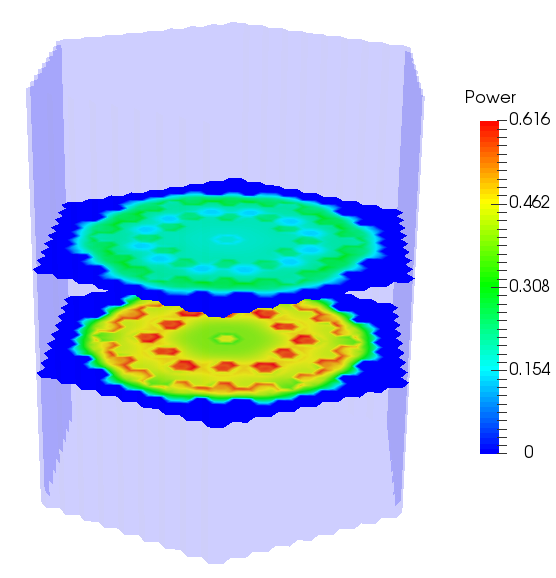
\includegraphics[width=1\linewidth]{u1h.png}} \\
		\end{minipage}
		\hfill
		\begin{minipage}{0.49\linewidth}
			\center{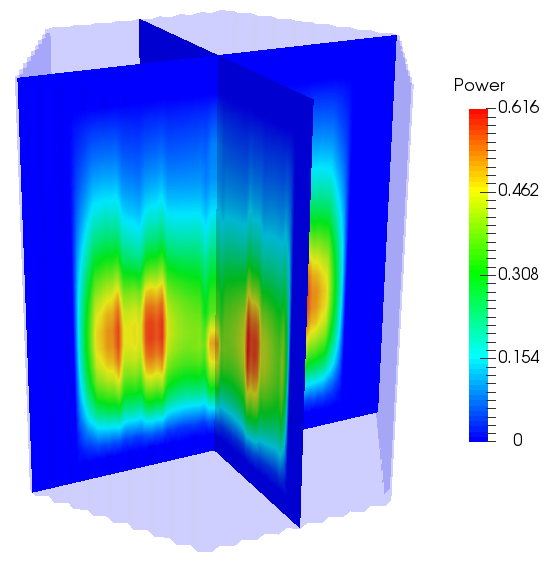
\includegraphics[width=1\linewidth]{u1v.png}} \\
		\end{minipage}
	\end{center}
\end{figure}
\end{frame}

\begin{frame}{Vertical and horizontal cuts for $k_2$}
\begin{figure}[!h]
	\begin{center}
		\begin{minipage}{0.49\linewidth}
			\center{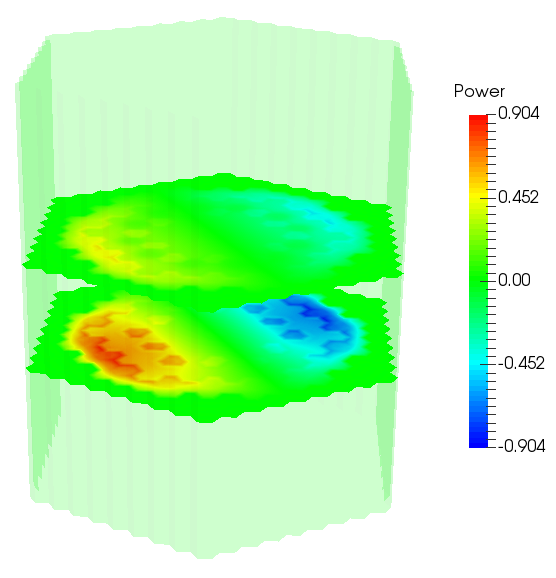
\includegraphics[width=1\linewidth]{u2h.png}} \\
		\end{minipage}
		\hfill
		\begin{minipage}{0.49\linewidth}
			\center{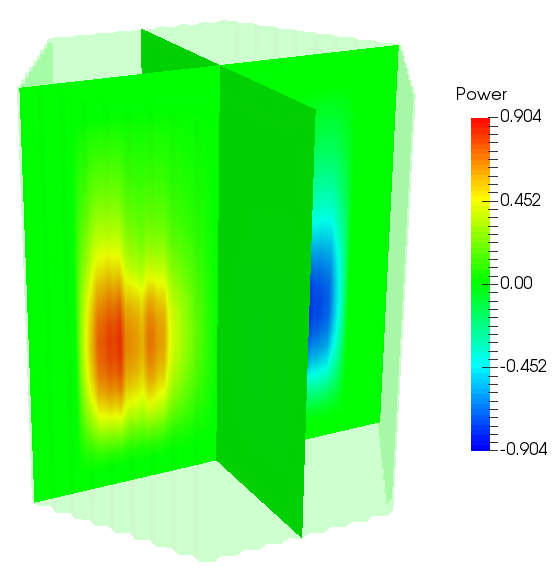
\includegraphics[width=1\linewidth]{u2v.png}} \\
		\end{minipage}
	\end{center}
\end{figure}
\end{frame}

\begin{frame}{Vertical and horizontal cuts for $k_3$}
\begin{figure}[!h]
	\begin{center}
		\begin{minipage}{0.49\linewidth}
			\center{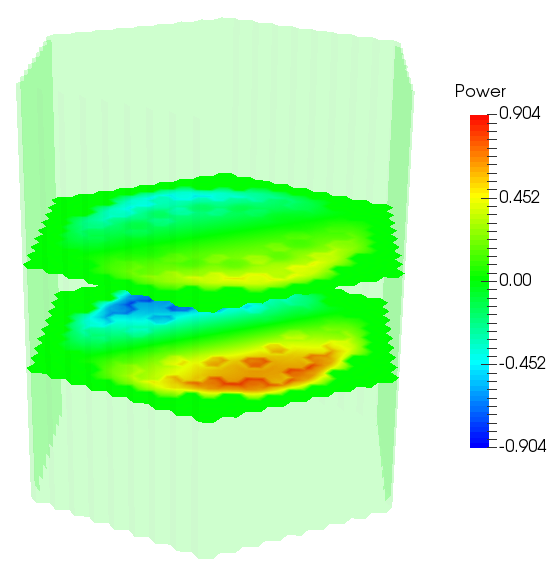
\includegraphics[width=1\linewidth]{u3h.png}} \\
		\end{minipage}
		\hfill
		\begin{minipage}{0.49\linewidth}
			\center{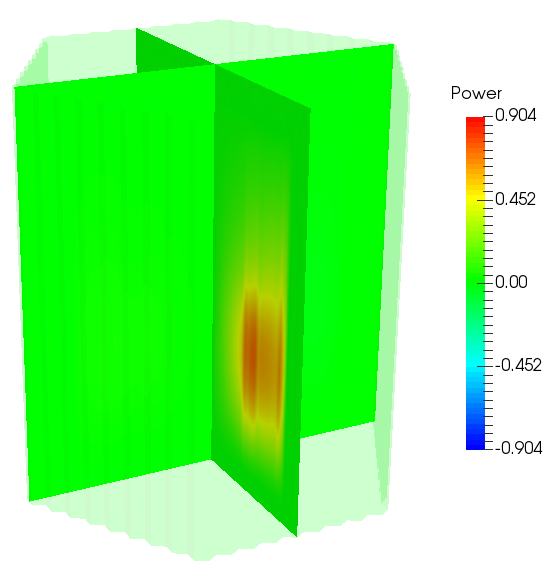
\includegraphics[width=1\linewidth]{u3v.png}} \\
		\end{minipage}
	\end{center}
\end{figure}
\end{frame}

\begin{frame}{Vertical and horizontal cuts for $k_4$}
\begin{figure}[!h]
	\begin{center}
		\begin{minipage}{0.49\linewidth}
			\center{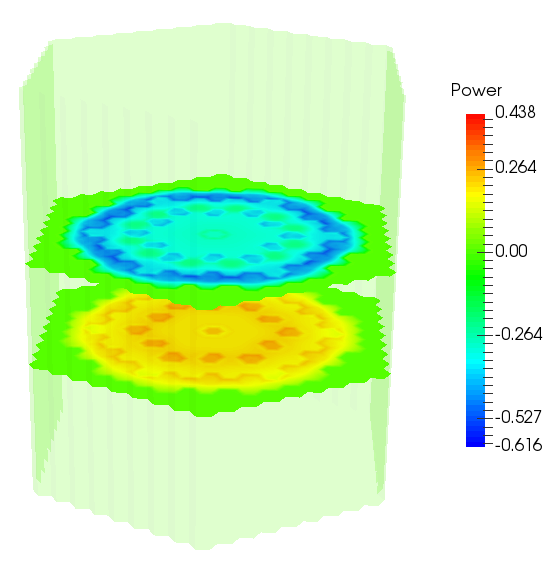
\includegraphics[width=1\linewidth]{u4h.png}} \\
		\end{minipage}
		\hfill
		\begin{minipage}{0.49\linewidth}
			\center{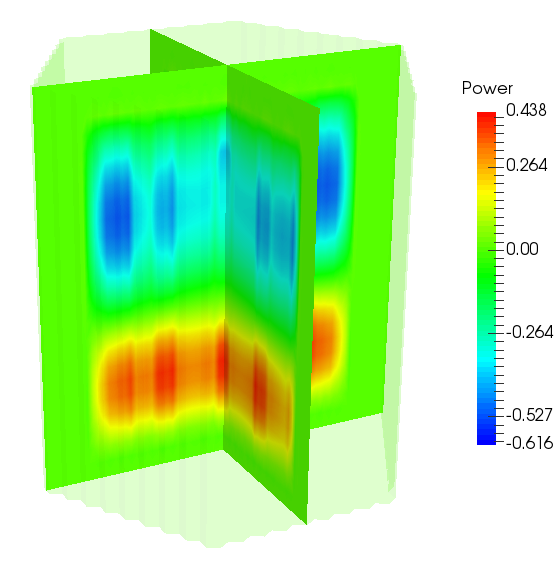
\includegraphics[width=1\linewidth]{u4v.png}} \\
		\end{minipage}
	\end{center}
\end{figure}
\end{frame}

\section{Conclusion}
\begin{frame}{Conclusion}
In this paper we have performed computational analysis of the 3D neutron diffusion benchmark of a VVER-1000 core. The software has been developed using the engineering and scientic library FEniCS and the matrix spectral problem is solved using the SLEPc package. The number of tetrahedrons per assembly $\kappa$ varies from 6 to 96; the number of tetrahedrons in height $z$ varies from 12 to 48. The finite elements of degree $p$ = 1, 2, 3 are used. The results are compared with the extrapolated finite-element solution of the second-order CRONOS results recommended as the reference solution. An excellent agreement of the results was obtained for the maximum values of the parameters ($\kappa$=96, $z$=48 and $p$=3). There are deviations in the results at the rounding error level. In the practice of engineering calculations it is sufficient to use the following parameters: $\kappa$=6, $z$=24 and $p$=2. The results can be useful for the diffusion codes intercomparison.

\begin{center}
Thank you for your attention!
\end{center}
\end{frame}

\end{document}
